%%%%%%%%%%%%%%%%%%%%%%%%%%%%%%%%%%%%%%%%%
% Short Sectioned Assignment
% LaTeX Template
% Version 1.0 (5/5/12)
%
% This template has been downloaded from:
% http://www.LaTeXTemplates.com
%
% Original author:
% Frits Wenneker (http://www.howtotex.com)
%
% License:
% CC BY-NC-SA 3.0 (http://creativecommons.org/licenses/by-nc-sa/3.0/)
%
% Download template:
% Overleaf (https://www.overleaf.com/8746855dtrgkbkbjjhm)
%
%%%%%%%%%%%%%%%%%%%%%%%%%%%%%%%%%%%%%%%%%

%-------------------------------------------------------------------------------
%	PACKAGES AND OTHER DOCUMENT CONFIGURATIONS
%-------------------------------------------------------------------------------

%\documentclass[paper=a4, fontsize=11pt]{scrartcl} % A4 paper and 11pt font size
\documentclass[a4paper]{article}
%\documentclass[11pt]{article}
%\usepackage[margin=1.25in]{geometry}

%\usepackage[options]{nohyperref}  % This makes hyperref commands do nothing without errors
%\usepackage{url}  % This makes \url work
%\usepackage{hyperref}

\usepackage{graphicx}

%\usepackage[T1]{fontenc} % Use 8-bit encoding that has 256 glyphs
\usepackage[utf8]{inputenc}
%\usepackage{fourier} % Use the Adobe Utopia font for the document - comment this line to return to the LaTeX default
\usepackage[english]{babel} % English language/hyphenation
\usepackage{mathtools,amsmath,amsfonts,amsthm} % Math packages
\usepackage{amssymb}

%\usepackage{lipsum} % Used for inserting dummy 'Lorem ipsum' text into the template

\usepackage{sectsty} % Allows customizing section commands
\allsectionsfont{\centering \normalfont\scshape} % Make all sections centered, the default font and small caps

\usepackage{fancyhdr} % Custom headers and footers
%\pagestyle{fancyplain} % Makes all pages in the document conform to the custom headers and footers
%\fancyhead{} % No page header - if you want one, create it in the same way as the footers below
%\fancyfoot[L]{} % Empty left footer
%\fancyfoot[C]{} % Empty center footer
%\fancyfoot[R]{\thepage} % Page numbering for right footer
\renewcommand{\headrulewidth}{0pt} % Remove header underlines
\renewcommand{\footrulewidth}{0pt} % Remove footer underlines
\setlength{\headheight}{13.6pt} % Customize the height of the header

\numberwithin{equation}{section} % Number equations within sections (i.e. 1.1, 1.2, 2.1, 2.2 instead of 1, 2, 3, 4)
\numberwithin{figure}{section} % Number figures within sections (i.e. 1.1, 1.2, 2.1, 2.2 instead of 1, 2, 3, 4)
\numberwithin{table}{section} % Number tables within sections (i.e. 1.1, 1.2, 2.1, 2.2 instead of 1, 2, 3, 4)

%\setlength\parindent{0pt} % Removes all indentation from paragraphs - comment this line for an assignment with lots of text
\usepackage{indentfirst} % Indentation for all paragraphs

% Used for definitions:
\usepackage{amsthm}
\theoremstyle{definition}
\newtheorem{definition}{Definition}[section]

% To write algorithms in pseudocode:
\usepackage{algpseudocode}
\usepackage{algorithm}

% Don't use colon in algorithms lines:
\algrenewcommand\alglinenumber[1]{\footnotesize #1}

% Input/Output instead of Require/Ensure in algorithms pseudocode:
\renewcommand{\algorithmicrequire}{\textbf{Input:}}
\renewcommand{\algorithmicensure}{\textbf{Output:}}

% To put images side by side:
\usepackage{subcaption}

% Avoid long sentences to go out of margines:
\usepackage{microtype}

% Use URL and avoid long urls to go out of margins (hyphens):
\usepackage[hyphens]{url}

% Define multiline to avoid unindented long sentences in algorithms:
% (https://tex.stackexchange.com/questions/314023/how-to-indent-a-long-sentence-in-an-algorithm)
\usepackage{tabularx}
\makeatletter
\newcommand{\multiline}[1]{%
  \begin{tabularx}{\dimexpr\linewidth-\ALG@thistlm}[t]{@{}X@{}}
    #1
  \end{tabularx}
}
\makeatother

%-------------------------------------------------------------------------------
%	TITLE SECTION
%-------------------------------------------------------------------------------

\newcommand{\horrule}[1]{\rule{\linewidth}{#1}} % Create horizontal rule command with 1 argument of height

\title{
\normalfont \normalsize
\textsc{Sapienza University of Rome} \\ [25pt] % Your university, school and/or department name(s)
\horrule{0.5pt} \\[0.4cm] % Thin top horizontal rule
\LARGE Artificial Intelligence \\ % The assignment title
\large Solving Pong using Deep-Q Learning \\
\horrule{2pt} \\[0.5cm] % Thick bottom horizontal rule
}

\author{Michele Cipriano} % Your name

\date{\normalsize\today} % Today's date or a custom date

\begin{document}
\sloppy % avoid to make words to go out of margin

\maketitle % Print the title

%-------------------------------------------------------------------------------

\section{Introduction}

In the last years, reinforcement learning has seen an increasing interest thanks,
in particular, to GPUs and the diffusion of deep learning. The aim of this
project is to study the Deep-Q Learning with Experience Replay
algorithm, introduced in \cite{mnih2013playing}, and train
a Deep-Q Network on the game of Pong, using OpenAI Gym environments\cite{openai-gym}.

In particular, different experiments have been performed comparing the algorithm
of \cite{mnih2013playing} and its successor, introduced in the famous Nature
paper \cite{mnih2015humanlevel}. The networks have been trained on two different
Pong environments, which differs in the way the agent interacts with the them.

The project has been developed entirely in Python, using TensorFlow to define and
train the neural networks and Gym to interact with the Atari Pong environments.
The training phase has been performed on Google Compute Engine, which provides an
easy access to GPU computational power.

The experiments have been done on two slightly different Pong environments.
The best network obtained a maximum average score (averaged over 25 episodes) of
16.96 on \texttt{PongNoFrameskip-v0} learning a good
strategy just after 600,000 frames.

%-------------------------------------------------------------------------------

\section{Gym}

OpenAI Gym is a toolkit for reinforcement learning research which includes a
collection of environments. The environments share a common interface with which
the agent can interact. In particular, at each timestep, the agent performs an
action receiving an observation, a reward and a boolean value telling whether the
observation is final with respect to the episode or not.

Part of this environments are classic Atari games and make use of Arcade Learning
Environment. This project makes use of two similar Pong environments,
\texttt{Pong-v0} and \texttt{PongNoFrameskip-v0}. Both returns as observation
an RGB image of shape $(210, 160, 3)$. The difference is within the number of times
the action is repeated: while in \texttt{Pong-v0} each action is repeatedly
performed for a duration of $k$ frames, where $k$ is uniformely sampled from
$\{ 2, 3, 4 \}$, in \texttt{PongNoFrameskip-v0} each action is performed only for
a single frame.

Another interesting tool used in this project are OpenAI Atari
wrappers\cite{openai-gym-baselines}, which simplify the management of the frames,
providing preprocessing and different levels of abstraction on the observations.
The main wrappers used are:
\begin{itemize}
	\item \textbf{WarpFrame}: warp frame to $84 \times 84$ as done in \cite{mnih2015humanlevel}.
	\item \textbf{FrameStack}: stack $k$ last frames, this wrapper is used to
		obtain tensors of size $84 \times 84 \times 4$ that can be easily fed to the DQN.
	\item \textbf{MaxAndSkipEnv}: return an observation only every $k$-th frame. This wrapper has
		been used only with \texttt{PongNoFrameskip-v0} to speed up training by repeating
		the same action $k=4$ times, reducing stochasticity w.r.t. \texttt{Pong-v0}.
\end{itemize}

%-------------------------------------------------------------------------------

\section{Deep-Q Learning}

Let's consider a task in which an agent interacts with an environment $\mathcal{E}$,
in this case an Atari emulator with the Pong game, by taking at each timestep $t$
an action $a_t$ from a set of action $ \mathcal{A} = \left\{ 1, \dots, K \right\} $.
After the action has been performed, the agent observes
an image $x_t \in \mathbb{R}^d$ and receives a reward $r_t$, representing the
change in the game score.

Let's consider finite sequences of actions and observations $s_t = x_1, a_1, x_2, \dots,
a_{t-1}, x_t$ for each timestep $t$ and define a Markov Decision Process (MDP) where
each sequence is a distinct state. The future discounted reward
at time $t$, defined as $R_t = \sum_{t'=t}^{T} \gamma^{t'-t} r_{t'}$, where $\gamma$ is the
discount factor can be used to define the optimal action-value function:
\begin{equation*}
	Q^*(s, a) = \max_\pi \mathbb{E} \left[ R_t \mid s_t = s, a_t = a, \pi \right]
\end{equation*}

\noindent where $\pi$ is a policy mapping sequences to actions. Since this function
can also be defined by using the \textit{Bellman optimality equation}:
\begin{equation*}
	Q^*(s, a) = \mathbb{E}_{s' \sim \mathcal{E}} \left[ r + \gamma \max_{a'} Q^*(s', a') \middle| s, a \right]
\end{equation*}

\noindent it is possible to estimate it by using an iterative update:
\begin{equation*}
	Q_{i+1}(s, a) = \mathbb{E}_{s' \sim \mathcal{E}} \left[ r + \gamma \max_{a'} Q_{i}(s', a') \middle| s, a \right]
\end{equation*}

\noindent converging to the optimal action-value function $Q_i \rightarrow Q^*$
as $i \rightarrow \infty$. Of course, when the state space is too big, like
in the case of Pong, it is impossible to store all the values in a single table.
Moreover, the iterative update would take too much time to converge since no
generalization is done on the problem. This problem can be easily handled by
approximating the Q function with a function $Q(s, a; \theta) \approx Q^*(s, a)$
which depends on the weights $\theta$. In this project $Q(s, a; \theta)$ has been
defined by using the deep neural networks (Q-network) described in
\cite{mnih2013playing} and \cite{mnih2015humanlevel}.

In the first experiment the neural network has been trained by minimizing
a sequence of loss functions that changes at each iteration $i$:
\begin{equation}
	\label{eq:loss-function-dqn13}
	L_i(\theta_i) = \mathbb{E}_{s, a \sim \rho(\cdot)} \left[ (y_i - Q(s, a; \theta_i))^2 \right]
\end{equation}

\noindent where $y_i = \mathbb{E}_{s' \sim \mathcal{E}} \left[ r + \gamma \max_{a'} Q(s', a'; \theta_{i-1}) \right]$,
$\rho(s, a)$ is the probability distribution over sequences $s$ and actions $a$
and $\theta_{i-1}$ are the parameters of the network at iteration $i-1$ which
are held fixed during the optimization step.

A simple strategy to replace the expectations and to simplify the computation
of the gradient of the
loss function (in order to perform the optimization) is to sample data from the
distribution $\rho$ and the emulator $\mathcal{E}$. This is done via a technique
called \textit{experience replay}, which consists in storing in a dataset
$\mathcal{D} = e_1, e_2, \dots, e_N$ the experience
$e_t = \left( s_t, a_t, r_t, s_{t+1} \right)$ of the agent at each timestep $t$.
This allows to perform each gradient descent step using a minibatch of experiences
$e \sim \mathcal{D}$
sampled from the experience replay dataset.

Let's now describe the Deep Q-learning with Experience Replay algorithm
(algorithm \ref{algorithm:deep-q-learning-13}) introduced in \cite{mnih2013playing}.
The main cycle executes $M$ episodes interacting with the Gym environment and
updating the weights $\theta$ of the neural network. First, the sequence is
initialized (line 4) with the first frame returned by the environment, which
is itself preprocessed by a function $\phi$ which makes it feedable to the neural
network. The function $\phi$, as described in \cite{mnih2013playing}, takes as
input a RGB frame of shape $(210, 160, 3)$ and return a frame of shape
$(84, 84, 1)$ after converting the input to a greyscale image, downsampling it
to a $(110, 84, 1)$ image and cropping an $(84, 84, 1)$ region that captures
the playing area. To maximize the performances of the program, the preprocessing
has been done with the OpenAI Atari Wrappers\cite{openai-gym-baselines}, described
above, which also stack the last four observations (frames) returned by the environment.
The agent selects an action $a_t$ using an epsilon-greedy strategy (lines 6-7),
where $\epsilon$ is linearly descreased for the first 100,000 frames from $1.0$
to $0.02$, and executes it in the environment, receiving a reward $r_t$ and observing
an image $x_{t+1}$ (line 8). The sequence is preprocessed as described above and
the new transition is stored in the experience replay $\mathcal{D}$ (lines 9-10).
At this point a minibatch of transitions is sampled from $\mathcal{D}$ and it is
used to performed a gradient descent step on the loss function (lines 11-13).
Note that the target $y_j$ changes depending on the last observed
frame\footnote{The experience replay implementation also stores the boolean
\texttt{done}\ which denotes the end of the episode.} (if it is final or not).
To have a comparison with a fast convergence implementation (see \cite{Medium-Pong-30min}),
the optimization algorithm used has been Adam (with learning rate $\eta = 0.0001$)
instead of RMSProp as originally proposed in the paper, which has faster
convergence properties w.r.t RMSProp\cite{Adam-Kingma} even if it is less stable
in this scenario. The training has been started after 10,000 observations.

\begin{algorithm}
	\caption{Deep Q-learning with Experience Replay\cite{mnih2013playing}}
	\label{algorithm:deep-q-learning-13}
	\begin{algorithmic}[1]
    \State Initialize replay memory $\mathcal{D}$ to capacity $N$
    \State Initialize action-value function $Q$ with random weights $\theta$
		\For {episode = $1, M$}
			\State Initialize sequence $s_1 = \left\{ x_1 \right\}$ and preprocessed sequence $\phi_1 = \phi(s_1)$
			\For {$t = 1, T$}
				\State With probability $\epsilon$ select a random action $a_t$
				\State otherwise select $a_t = \max_a Q(\phi(s_t), a; \theta)$
				\State Execute action $a_t$ in emulator and observe reward $r_t$ and image $x_{t+1}$
				\State Set $s_{t+1} = s_t, a_t, x_{t+1}$ and preprocess $\phi_{t+1} = \phi(s_{t+1})$
				\State Store transition $(\phi_t, a_t, r_t, \phi_{t+1})$ in $\mathcal{D}$
				\State Sample random minibatch of transitions $(\phi_j, a_j, r_j, \phi_{j+1})$ from $\mathcal{D}$
				\State Set $ y_j =
									   \begin{cases}
									     r_j       & \quad \text{for terminal } \phi_{j+1}\\
									     r_j + \gamma \max_{a'} Q(\phi_{j+1}, a', \theta)  & \quad \text{for non-terminal } \phi_{j+1}
									   \end{cases}
									 $
				\State Perform a gradient descent step on $(y_j - Q(\phi_j, a_j; \theta))^2$
			\EndFor
		\EndFor
	\end{algorithmic}
\end{algorithm}

As said before, the function $Q$ is parametrized by a neural network.
Its architecture is pretty simple, it consists of a hidden layer which convolves
16 $8 \times 8$ filters with stride 4 applying nonlinearity through the rectified
linear unit ($ReLU(x) = \max(0, x)$), followed by another convolutional layer,
which convolves 32 $4 \times 4$ with stride 2 applying $ReLU$ nonlinearity, followed
by a fully connected layer of 512 $ReLU$ units\footnote{In the original paper the final
hidden layer has size 256.} and an output layer with a single output for each
valid action of the selected environment (6 in the case of Pong).

The network has been trained on the environment \texttt{Pong-v0} for 1,000 episodes (around 3M frames) using a
batchsize of 32 elements and a discount factor $\gamma = 0.99$ reaching
an average reward per episode (computed over 25 episodes) of $-4.84$ as it is
possible to see from figure \ref{fig:experiments}.

Let's now improve the algorithm by adding a target network and changing the loss
function and the architecture of the network as done in \cite{mnih2015humanlevel}.
The idea is to improve the training by improving the stability of the algorithm.

Let's change the definition of the loss function in \ref{eq:loss-function-dqn13}
by:
\begin{equation*}
	L_i(\theta_i) = \mathbb{E}_{s, a, r, s' \sim U(\mathcal{D})} \left[ L_{\delta}\left( r + \gamma \max_{a'} Q(s', a'; \theta_i^-) - Q(s, a; \theta_i) \right) \right]
\end{equation*}

\noindent where $U(\mathcal{D})$ is the uniform distribution describing the
experience replay, $\theta_i^-$ are the parameters of the target network, updated
only every $C$ steps and hence kept fixed during the optimization steps,
$\theta_i$ are the parameters describing the action-value function $Q$ (note that
in algorithm \ref{algorithm:deep-q-learning-15} the target network is denoted
as $\hat{Q}$) and $L_{\delta}$ is the Huber loss function, defined as:
\begin{equation*}
	L_{\delta}(a) =
		\begin{cases}
		 \frac{1}{2}a^2 & \quad \text{for } |a| \le \delta \\
		 \delta \left( |a| - \frac{1}{2}\delta \right) & \quad \text{otherwise}
		\end{cases}
\end{equation*}

\noindent which behaves quadratically for small values of $a$ and linearly for
larger values. The architecture of the action-value function $Q$ is similar to
the one described above. It consists of a convolutional layer which convolves
32 $8 \times 8$ filters with stride 4 applying $ReLU$ nonlinearity, followed by
another convolutional layer which convolves 64 $4 \times 4$ filters with stride
2 applying $ReLU$, followed by a third convolutional layer which convolves
64 $3 \times 3$ filters with stride 1 applying again $ReLU$. The three convolutional
layers are followed by a fully connected layer of 512 $ReLU$ units and an output
layer of the size corresponding to the number of valid action of the environment.

The resulting algorithm (algorithm \ref{algorithm:deep-q-learning-15}), described below,
is similar to the previous one, except for the target action-value function $\hat{Q}$,
initialized on line 3, used to compute the target value $y_j$ on line 13 and updated
every $C$ steps on line 15, the weights $\theta^-$, that parametrize the function $\hat{Q}$,
and the loss function (line 14), which is the Huber loss instead of the squared
loss.

The network has been trained on the environment \texttt{Pong-v0} for 1,000 episodes (around 3.6M frames) using a
batchsize of 32 elements and a discount factor $\gamma = 0.99$ reaching
an average reward per episode (computed over 25 episodes) of $0.2$ as it is
possible to see from figure \ref{fig:experiments}. The Huber loss function
has been used with $\delta = 1$. Algorithm
\ref{algorithm:deep-q-learning-15} slightly improves algorithm
\ref{algorithm:deep-q-learning-13} performing much better in particular in the
initial phase, where the agent explores the environment more frequently.

\begin{algorithm}
	\caption{Deep Q-learning with Experience Replay\cite{mnih2015humanlevel}}
	\label{algorithm:deep-q-learning-15}
	\begin{algorithmic}[1]
    \State Initialize replay memory $\mathcal{D}$ to capacity $N$
    \State Initialize action-value function $Q$ with random weights $\theta$
		\State Initialize target action-value function $\hat{Q}$ with random weights $\theta^- = \theta$
		\For {episode = $1, M$}
			\State Initialize sequence $s_1 = \left\{ x_1 \right\}$ and preprocessed sequence $\phi_1 = \phi(s_1)$
			\For {$t = 1, T$}
				\State With probability $\epsilon$ select a random action $a_t$
				\State otherwise select $a_t = \max_a Q(\phi(s_t), a; \theta)$
				\State Execute action $a_t$ in emulator and observe reward $r_t$ and image $x_{t+1}$
				\State Set $s_{t+1} = s_t, a_t, x_{t+1}$ and preprocess $\phi_{t+1} = \phi(s_{t+1})$
				\State Store transition $(\phi_t, a_t, r_t, \phi_{t+1})$ in $\mathcal{D}$
				\State Sample random minibatch of transitions $(\phi_j, a_j, r_j, \phi_{j+1})$ from $\mathcal{D}$
				\State Set $ y_j =
									   \begin{cases}
									     r_j       & \quad \text{for terminal } \phi_{j+1}\\
									     r_j + \gamma \max_{a'} \hat{Q}(\phi_{j+1}, a', \theta^-)  & \quad \text{for non-terminal } \phi_{j+1}
									   \end{cases}
									 $
				\State \multiline{Perform a gradient descent step on $L_{\delta}(y_j - Q(\phi_j, a_j; \theta))$ w.r.t. the parameters $\theta$}
				\State Every $C$ steps reset $\hat{Q} = Q$
			\EndFor
		\EndFor
	\end{algorithmic}
\end{algorithm}

The same network has been trained with the same hyperparameters on a similar
Pong environment (\texttt{PongNoFrameskip-v0}), with the \texttt{MaxAndSkipEnv}
wrapper, resulting in a less stochastic environment than \texttt{Pong-v0}. As
said before, while in \texttt{Pong-v0} each action is performed randomly for 2, 3
or 4 frames, in \texttt{PongNoFrameskip-v0} each action is performed only once
for each frame. Combining this environment with \texttt{MaxAndSkipEnv} it has been
possible recreate the environment used in the Nature paper, executing the
same action for $k$ frames (in the experiment $k=4$) and
making the agent observe only each $k$-th frame, exactly as done in \cite{mnih2013playing}
and \cite{mnih2015humanlevel}. The network obtained an average reward per episode
of 16.96 (again, average over 25 episodes) analizing 3.3M frames (1,500 episodes).
It is interesting to notice that the network learns a good action-value function
in the first 600,000 frames, slightly improving until the end of the training process.

\begin{figure}
	\centering
	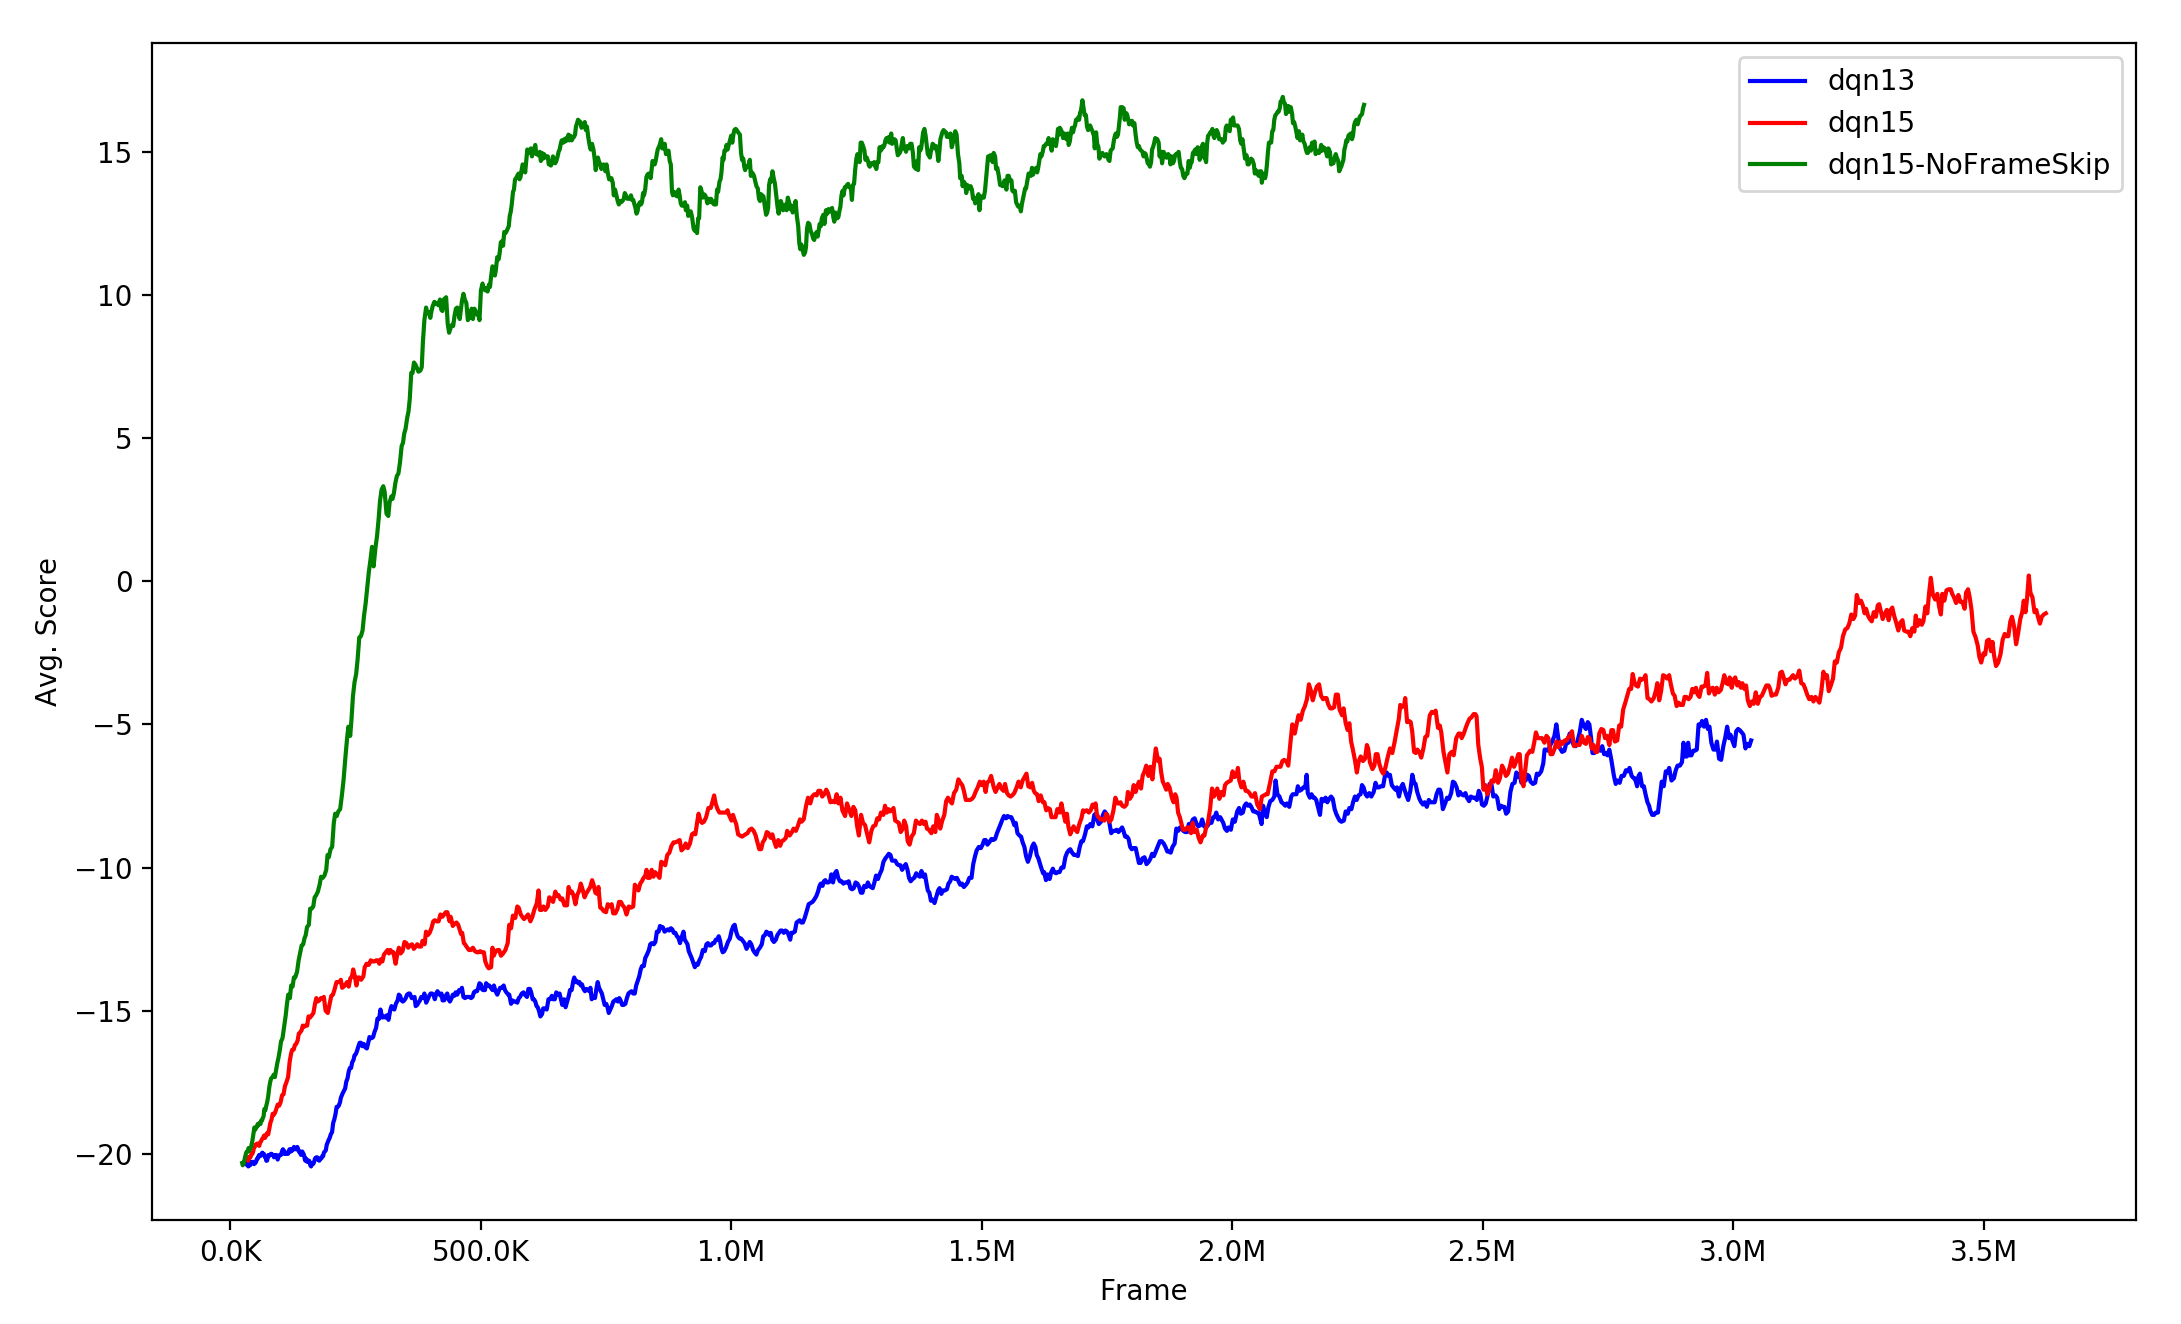
\includegraphics[width=1.0\linewidth]{images/dqn-results-pong.png}
	\caption{The figure shows the average score (averaged over 25 episodes) of
		the three described implementations. In blue the DQN of \cite{mnih2013playing}
		trained on \texttt{Pong-v0}.
		In red the DQN of \cite{mnih2015humanlevel}, trained on
		\texttt{Pong-v0}. In green the DQN of \cite{mnih2015humanlevel} trained
		on \texttt{PongNoFrameskip-v0}.}
	\label{fig:experiments}
\end{figure}

%-------------------------------------------------------------------------------

\section{Conclusion}

Deep-Q learning is a simple and powerful method to solve reinforcement learning
problems. The experiments of Pong have shown not only how much important is to
improve learning algorithms, in this case by introducing a target network,
using a more stable loss function and redefining the convolutional neural network,
but also how stochasticity can affect the performances of the network.

The experience replay memory, which provides data to the network, plays an
important role in the training phase. Improving the way the data are sampled from this
memory (for example by prioritizing samples from which the network can learn
more\cite{DBLP:journals/corr/SchaulQAS15}) could make the training more efficient,
making the same network learn better action-value functions in less time.

Reinforcement learning is a hot research topic and more and more methods are
introduced every day. Parallelizing the computation is essential in order to speed
up training and explore the environment quickly. Exploiting the structure of the
network by combining value-based and policy-based methods, like in actor-critic
methods\cite{mnih2016asynchronous}, seems to improve algorithms like Deep-Q
learning, even without the use of GPUs. For sure, the combination of both
GPUs and actor-critic methods will further improve current algorithms, making them
converge faster and with more
stability\cite{babaeizadeh2016ga3c, DBLP:journals/corr/abs-1802-01561}.

%-------------------------------------------------------------------------------

\newpage
\bibliography{bibliography}
\bibliographystyle{ieeetr}

%-------------------------------------------------------------------------------

\end{document}
\grid
\grid
